\section{\name Software Library} \label{sec:software}


We now describe the software implementation that realizes the framework described in the previous section. Figure~\ref{fig:arch} presents the high-level system design: the data layer is an immutable time-sorted coordinate format (COO) storage with lightweight graph views for efficient slicing; the execution layer is built around a hook manager that transparently performs complex transformations (e.g., temporal neighbors); and the ML layer materializes batches on-device for model computation. This separation of concerns yields workflows that are efficient and extensible, as we show in Section~\ref{sec:research_exp}.


\textbf{IO Adaptors and Data Preprocessing.} \name streamlines experimentation by integrating the widely-used benchmark dataset: TGB~\citep{huang2023temporal,tgb2}, in the form of IO Adapters, including loading, preprocessing, and train/validation/test splits. This allows researchers to start experiments immediately and compare models consistently with minimal overhead. Custom adapters are also supported via CSV and Pandas. Our design makes it straightforward to incorporate new benchmarks while ensuring consistent evaluation across all datasets (see Appendix~\ref{app:data}).

\textbf{Graph Storage and Graph Views.} The storage exposes an interface for graph queries, implemented using a time-sorted COO with a cached index. This enables binary search over timestamps, which is critical for recent-neighbor retrieval. The backend is designed for extension, allowing alternative layouts~\citep{lpma, gpma} so future models can use the most efficient data structures for their workload. Backed by the storage, graph views provide lightweight, concurrency-safe access to temporal sub-graphs. Each view tracks time boundaries and encodes read-access through the time granularity abstraction. This enables \name to perform both CTDG and DTDG-style loading, making it straightforward to study the effects of snapshot resolutions, as illustrated in Section~\ref{sec:research_exp}. Our discretization is fully vectorized, enabling efficient snapshot creation, as demonstrated in Table~\ref{tab:discretization_latency}.

\begin{figure*}[t]
  \centering
  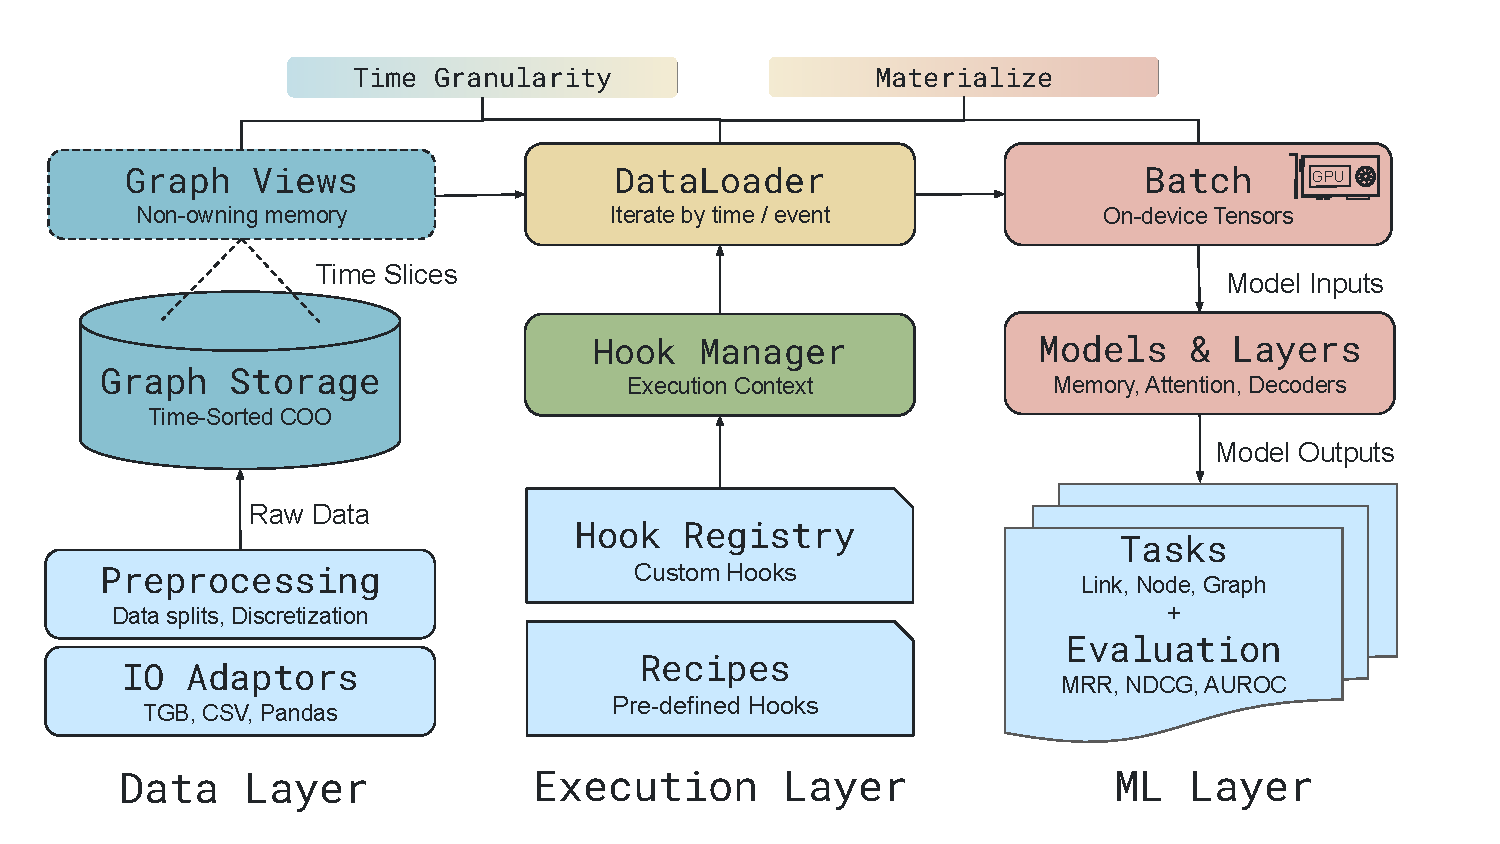
\includegraphics[width=0.9\linewidth]{iclr_2026/artifacts/architecture.pdf}
  % \includegraphics[width=0.95\linewidth]{iclr_2026/artifacts/TGM_overview.pdf}
  \caption{Three Layer Architecture of \name: data layer (left), with IO adaptors and preprocessing, immutable COO graph storage, and lightweight sub-graph views; execution layer (middle), where users register custom hooks or apply pre-built recipes through the hook manager and dataloader to inject execution logic; and ML layer (right), where batches are materialized on device and used for node-, link-, or graph-level prediction. Light blue elements denote user-facing APIs.}
  \label{fig:arch}
  % \vspace{-5mm}

\end{figure*}



\textbf{Hook Registry and Management.}
Building on the graph abstractions, hooks are transformations that can be combined to create complex workflows (see Section s~\ref{sec:tgm_frame}). The HookManager handles shared state, resolves dependencies, and executes transparently during data loading. A key-value interface allows hooks to be registered under specific conditions (e.g., analytics hooks, training hooks). We provide pre-defined recipes for common tasks such as TGB link prediction, helping new practitioners avoid common pitfalls like mismanaging state across data splits or using incorrect negatives.

\textbf{Diverse Model and Task Support.}
\name provides PyTorch modules tailored for TGL, including memory units, attention layers, and link decoders. With this, \name implements a range of TG methods, from baselines like EdgeBank~\citep{edgebank}, to message passing-based models like TGAT~\citep{tgat}, and frontier models like DyGFormer~\citep{dygfomer} and TPNet~\citep{tpnet}. Crucially, learnable components are decoupled from graph management, making it easy for researchers to prototype new models.


\begin{figure*}[!ht]
  \centering
  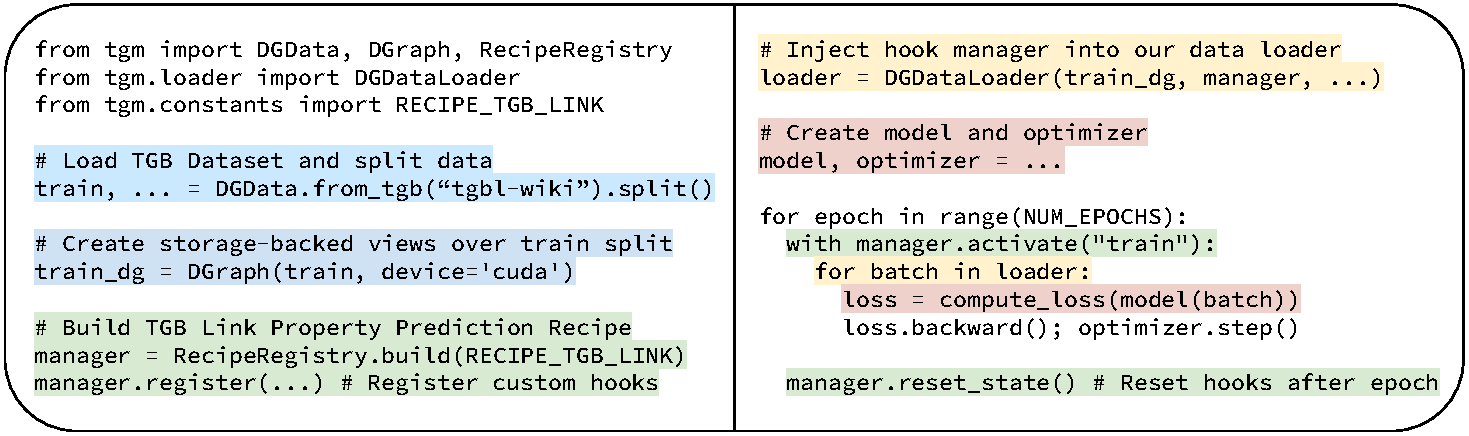
\includegraphics[width=0.9\linewidth]{iclr_2026/artifacts/code.pdf}
  \caption{Example workflow in \name. Left: dataset loading, graph creation, and hook registration; Right: manager injection, model setup, and training loop with automatic hook activation. Highlighted code maps to system components from Figure~\ref{fig:arch}.}
  \label{fig:workflow}
\end{figure*}


\textbf{Streamlined TGL Workflows.} Figure~\ref{fig:workflow} provides a high-level overview of a typical workflow in \name, illustrating how data preparation, graph creation, hook registration, and model training are orchestrated. Loading a temporal graph is straightforward, and hook registration can be shared and reused across different workflows, enabling code reuse. Registered hooks dynamically inject behaviour during data loading, ensuring models automatically receive the appropriate tensors. This unifies the model interface and explicitly defines which batch attributes each model consumes. The manager’s reset method exposes a single API for clearing the state of all active hooks. More complex workflows can be implemented by registering hooks under key-value pairs.


\textbf{Robust and Research-Ready Infrastructure.}
Finally, \name is built following modern software engineering practices to ensure reliability, maintainability, and ease of use. We use type hinting throughout the codebase, which unifies model APIs and improve usability. Continuous integration pipelines run end-to-end tests on all layers, hooks, and graph APIs with test coverage to ensure correctness. Performance monitoring utilities can track GPU usage with support for tools such as FlameProf~\citep{flame} to help identify bottlenecks. We also provide detailed tutorials, documentation, and examples for link, node and graph tasks. Overall, TGM provides a high-quality, research-ready platform that lowers the barrier to TG research while supporting efficient experimentation.


% \begin{figure*}[t]
%   \centering
%   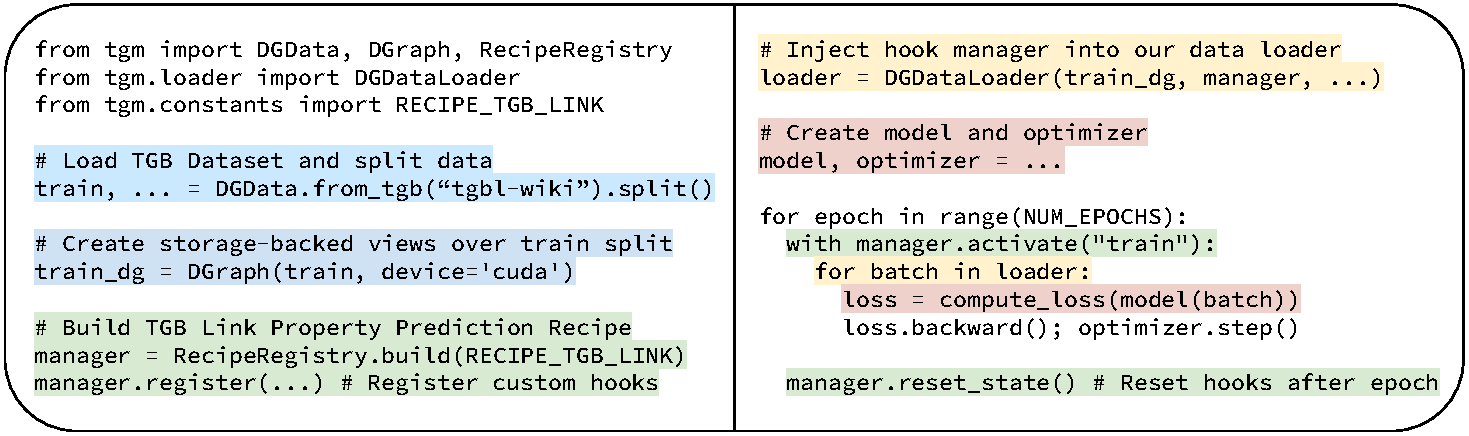
\includegraphics[width=0.9\linewidth]{iclr_2026/artifacts/code.pdf}
%   \caption{Example workflow in \name. Left: dataset loading, graph creation, and hook registration; Right: manager injection, model setup, and training loop with automatic hook activation. Highlighted code maps to system components from Figure~\ref{fig:arch}.}
%   \label{fig:workflow}
%   % \vskip -0.4in
% \end{figure*}
